
\documentclass[journal]{IEEEtran}
\usepackage{graphicx}
% *** MATH PACKAGES ***
%
\usepackage{amsmath}
% A popular package from the American Mathematical Society that provides
% many useful and powerful commands for dealing with mathematics.
%
% *** SPECIALIZED LIST PACKAGES ***
%
\usepackage{algorithmic}

% *** ALIGNMENT PACKAGES ***
%
\usepackage{array}
\usepackage[dvipsnames]{xcolor}
\usepackage{fancyvrb}

% redefine \VerbatimInput
\RecustomVerbatimCommand{\VerbatimInput}{VerbatimInput}%
{fontsize=\tiny,
 %
 frame=lines,  % top and bottom rule only
 framesep=2em, % separation between frame and text
 rulecolor=\color{Gray},
 %
 labelposition=topline,
 %
 commandchars=\|\(\), % escape character and argument delimiters for
                      % commands within the verbatim
 commentchar=*        % comment character
}
 \usepackage[caption=false,font=normalsize,labelfont=sf,textfont=sf]{subfig}

% *** PDF, URL AND HYPERLINK PACKAGES ***
%
\usepackage{hyperref}
\usepackage{url}

\hyphenation{op-tical net-works semi-conduc-tor}

\begin{document}
\title{Implemenation and Analysis of Tile Coloring Algorithm on CPU vs GPU}

\author{Joshua~Smith\\
        Utah State University\\
        joshua.smith4@aggiemail.usu.edu}

% The paper headers
\markboth{ECE 7720 - HW 1}{}

% make the title area
\maketitle

% As a general rule, do not put math, special symbols or citations
% in the abstract or keywords.
\begin{abstract}
This paper is an in depth analysis and discussion of the parallelization of a tile coloring algorithm implemented on a Tesla K80 Nvidia GPU. The serial algorithm is profiled and evaluated for the process of parallelization and then implemented two different ways. The first parallel implementation uses only GPU global memory and the second makes use of block shared memory. Each version is evaluated by its run time and speedup while varying the scheduling window size. The source code and results for this analysis can be found here: \url{https://github.com/joshua-smith4/ConcurrentNets}.
\end{abstract}

\IEEEpeerreviewmaketitle

\section{Introduction}

\IEEEPARstart{P}{arallelization} is the process of separating out parts of a serial algorithm that can be run concurrently with others. A \emph{general purpose graphics processing unit} (GPGPU) is specialized hardware that can run many threads simultaneously. In many areas of research and industry, massive speedup has been seen by parallelizing certain algorithms (e.g. sort, matrix multiplication, etc) on GPUs.

This paper focuses on the parallelization of the tile coloring problem. Two parallel implementation on a Tesla K80 Nvidia GPU demonstrate significant speedup over the serial algorithm. The first implemenation is rather naive with respect to memory accesses while the second utilizes block shared memory to further improve the algorithm.

\section{Familiarization with CUDA and GPU Device}

The first part of this project was getting familiar with the CUDA API for communicating with and launching kernels on the GPU. The results of the deviceQuery sample program shipped with CUDA detail the precise specifications of the GPU used and are included in Appendix A.

The following are a few key features to note about the device:
\begin{itemize}
  \item 11440 MB Global Memory
  \item 49 KB shared memory per block
  \item 1024 threads per block
  \item Max thread block dimensions (1024, 1024, 64)
\end{itemize}

Another sample program that tests the memory bandwidth of the device was run and the results are included in Appendix B. Figure \ref{fig:bandwidth} shows the memory bandwidth for varying data transfer sizes from device to device, host to device, and device to host.

\begin{figure}[ht]
\centering
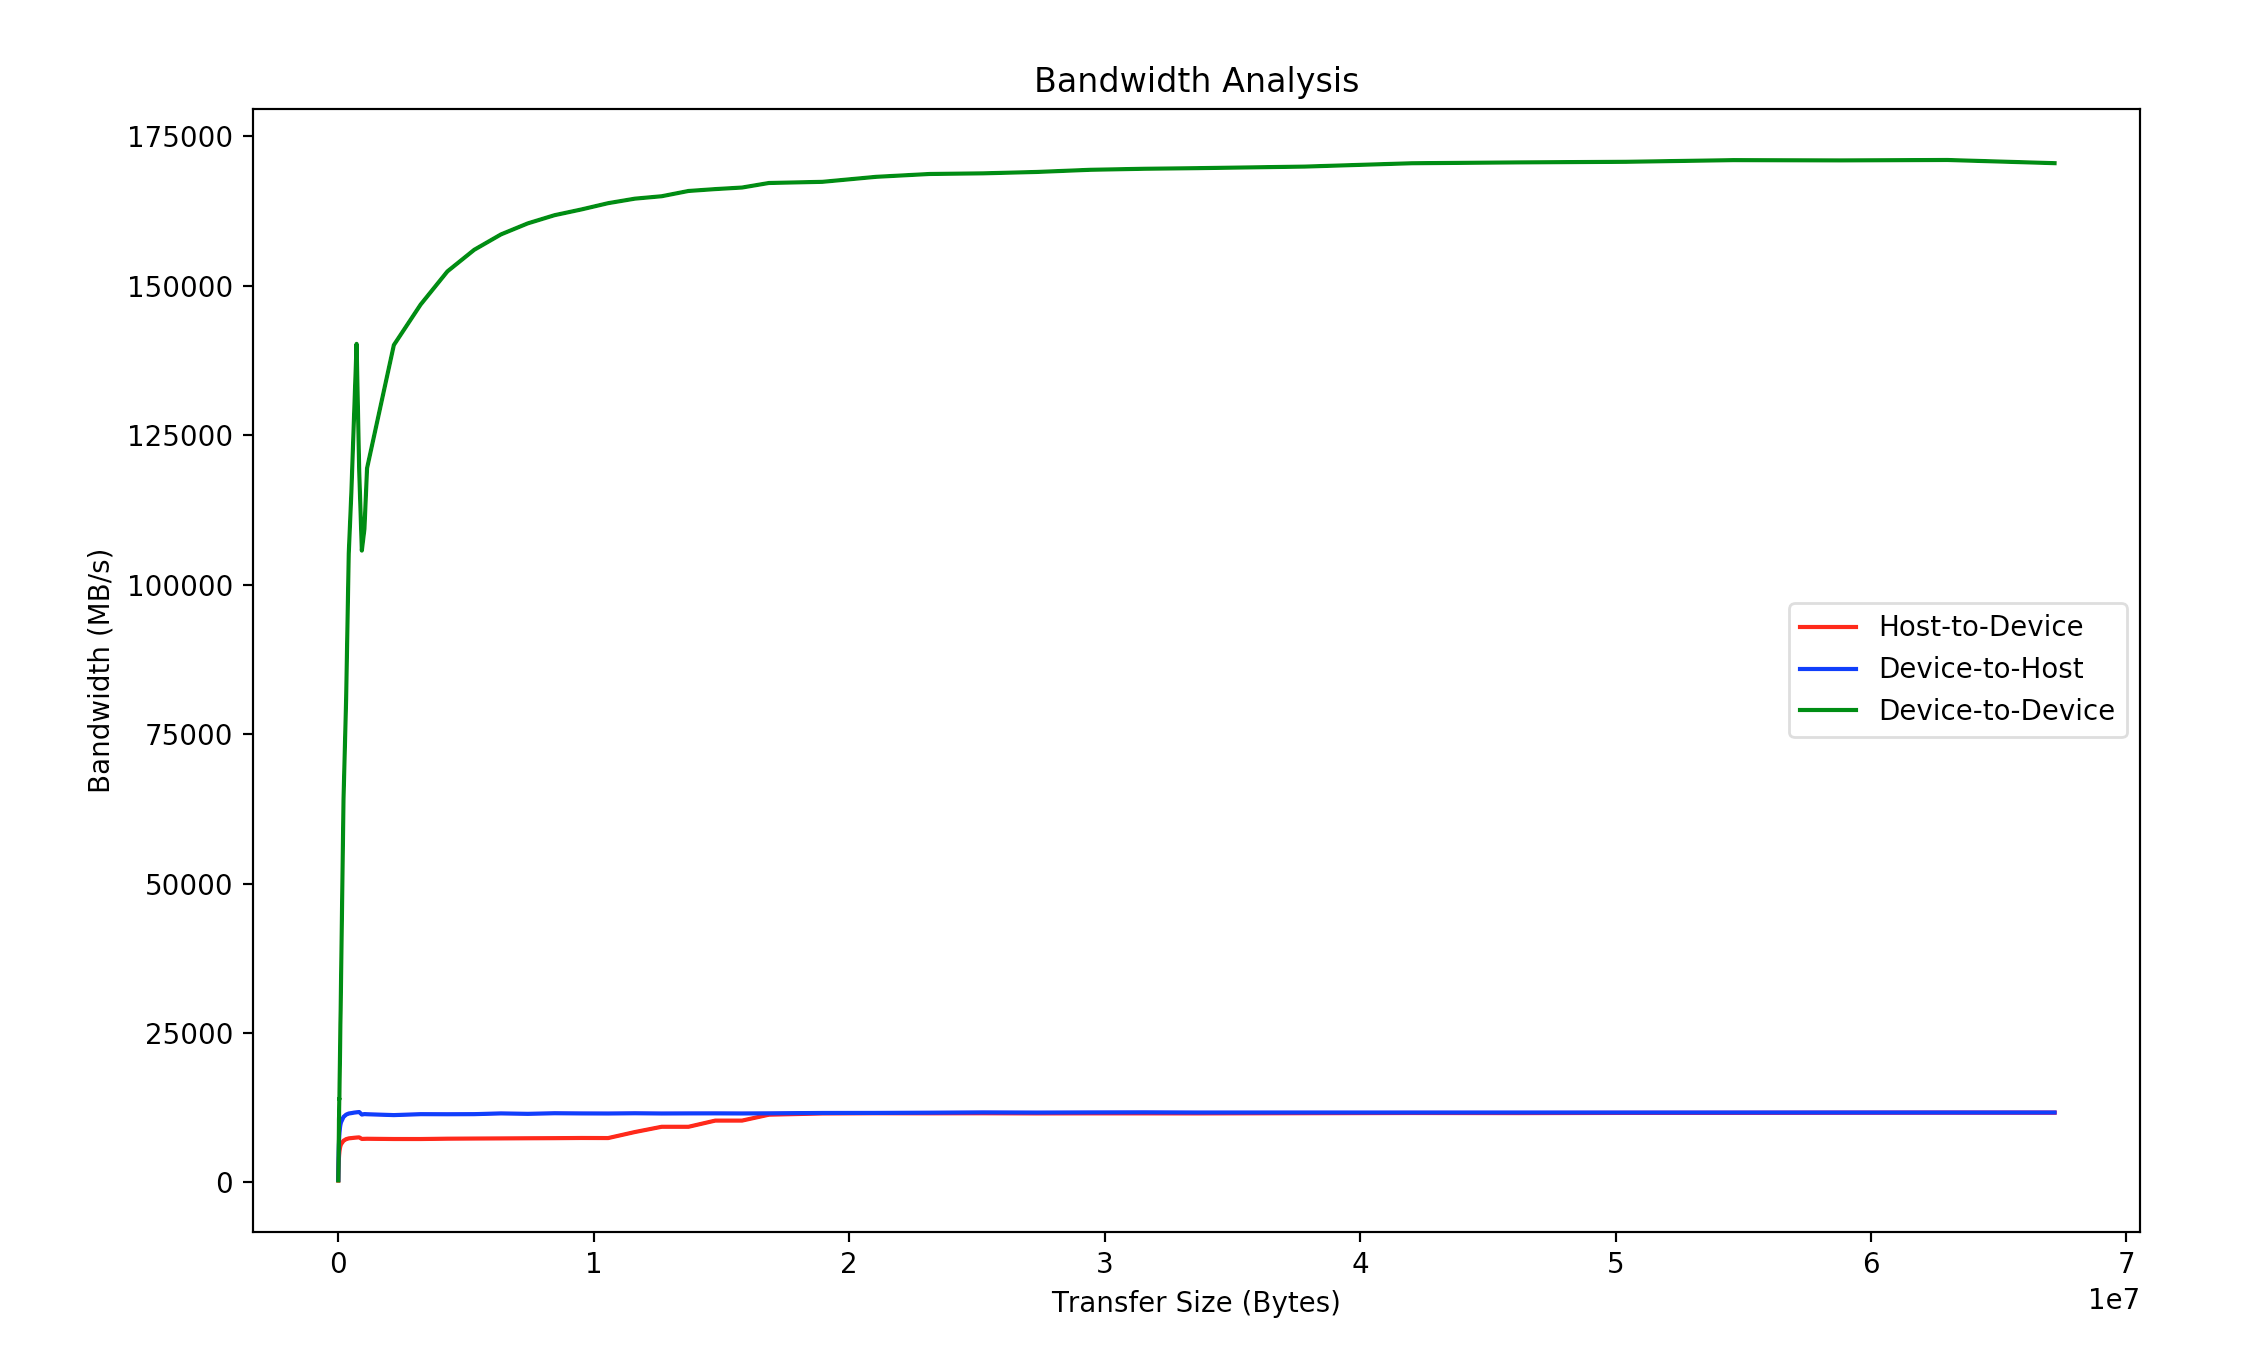
\includegraphics[width=0.5\textwidth]{bandwidth_analysis}
\caption{Bandwidth measurements of varying data transfer sizes between devices and host.}
\label{fig:bandwidth}
\end{figure}

\section{CPU Analysis and Parallel Design}

Per Amdahl's law, the potential speedup of an algorithm depends greatly on the size of the parallelizable portion. The tile coloring problem must be evaluated for speed up potential in order to justify the effort of parallelizing the portions that can be run concurrently. Figure \ref{fig:cpu_time} shows the amount of time spent per function on the serial algorithm. As can be seen, the function \emph{findConcurrencyCPU} takes up about 98\% of the algorithm's time. If this portion of code can be serialized, the resulting speedup would be very large and the effort is justified according to Amdahl's law.

\begin{figure}[ht]
\centering
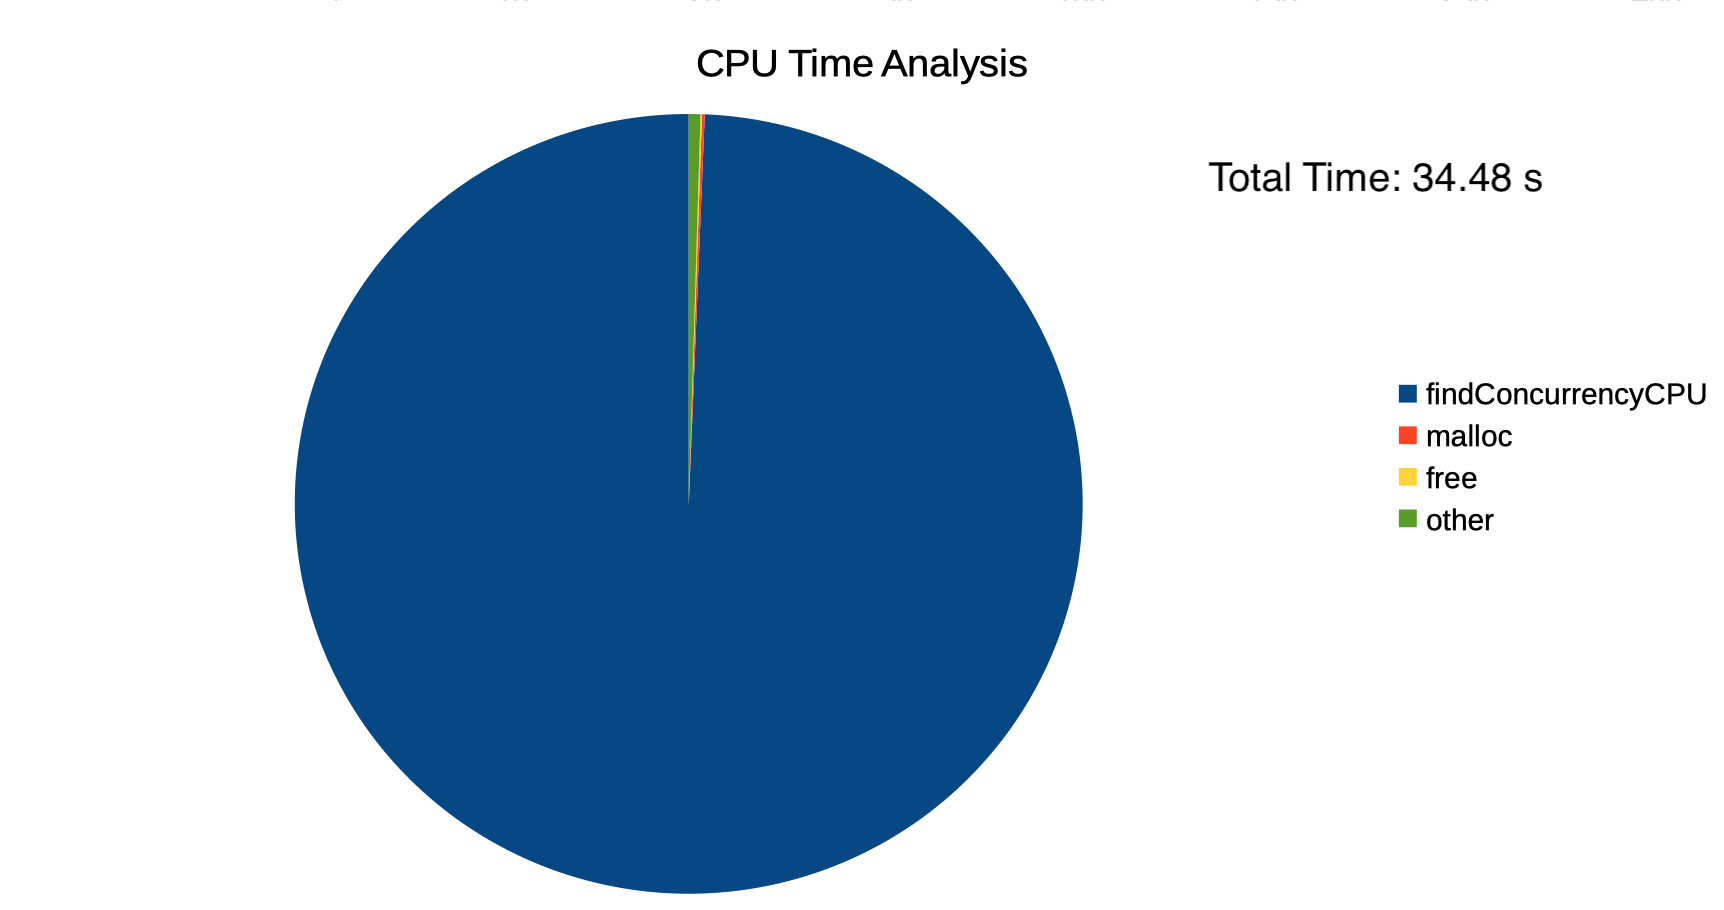
\includegraphics[width=0.5\textwidth]{cpu_time_analysis}
\caption{Time analysis of serial algorithm executed on the CPU.}
\label{fig:cpu_time}
\end{figure}

\section{Methods}

The function \emph{findConcurrencyCPU} essentially has two steps that take a lot of CPU time. The first is the coloring of the tiles. There is essentially zero data dependency between each iteration of the nested for loop structure that performs this function, making it easily and readily parallelizable. This was trivially done by alloting a thread on the GPU for each iteration of the for loop and allowing the thread to update the color of the tile associated with it. The next section goes into greater detail of how shared memory was utilized to further improve the performance of this section.

The second part of the function \emph{findConcurrencyCPU} is essencially a histogram operation where a bin associated with a color or subnet is incremented as a nested for loop structure iterates over the now colored tiles. In general, the number of colors or subnets is much smaller than the number of tiles, meaning that, in a parallel environment, many threads would be attempting to increment the same memory locations. This introduces possible data races between threads that must be handled. This part is also parallelizable but several precautions have to be made in order to retain safety and increase efficiency.

The CUDA API has a function called atomicAdd which is an indivisible operation that increments the value at a provided memory location by the argument. This guarantees that no race conditions can occur between threads desiring to increment the same location in the histogram. This solves the race condition problem but introduces a bottleneck into the program. Because there are many more tiles than colors, in general, many threads attempt to increment the same bins simultaneously resulting in a lot of thread communication and waiting. This is undesirable as it decreases the effectiveness of the parallelization.

In order to overcome this issue, several copies of the bins were made and only certain threads, based on their indices, would were allowed to access each copy. By significantly increasing the number of memory locations, the probability of collisions sharply decreased, allowing the algorithm to continue approximately fully parallelized. After each copy was updated, the results were trivially gathered by another kernel whose objective was to accumulate the values in each bin copy.

Three kernel functions were used, each with the functions described above.
\begin{enumerate}
  \item colorTiles - color the tiles
  \item histCalc - calculate the histogram using many copies of the bin array
  \item sumHist - accumulated the values of the distributed histograms
\end{enumerate}

More detailed implementation specifications can be found in the source code here: \url{https://github.com/joshua-smith4/ConcurrentNets}. Also in this repository are the nvvp profiler files containing data gathered on each version of the algorithm. The git repository contains two branches \emph{gpu_noshared} and \emph{gpu_shared} that point to the respective versions of the source code. To reproduce the results, clone the repository, checkout the desired branch, build the source code and run the commands detailed in the README.

\section{Shared Memory vs Global Memory Implemenations}

As mentioned above, in the color the tiles section of the algorithm there are two arrays that all threads refer to often to evaluate the color of the tile. The first implementation stores these arrays, called $a$ and $b$ in global memory where each access is costly. The second implementation first copies these arrays into shared memory, synchronizes threads in the block, then uses the shared memory to evaluate the tile color. This change resulted in a the speedups shown in Figure \ref{fig:globalvshared}.

\begin{figure}[ht]
\centering
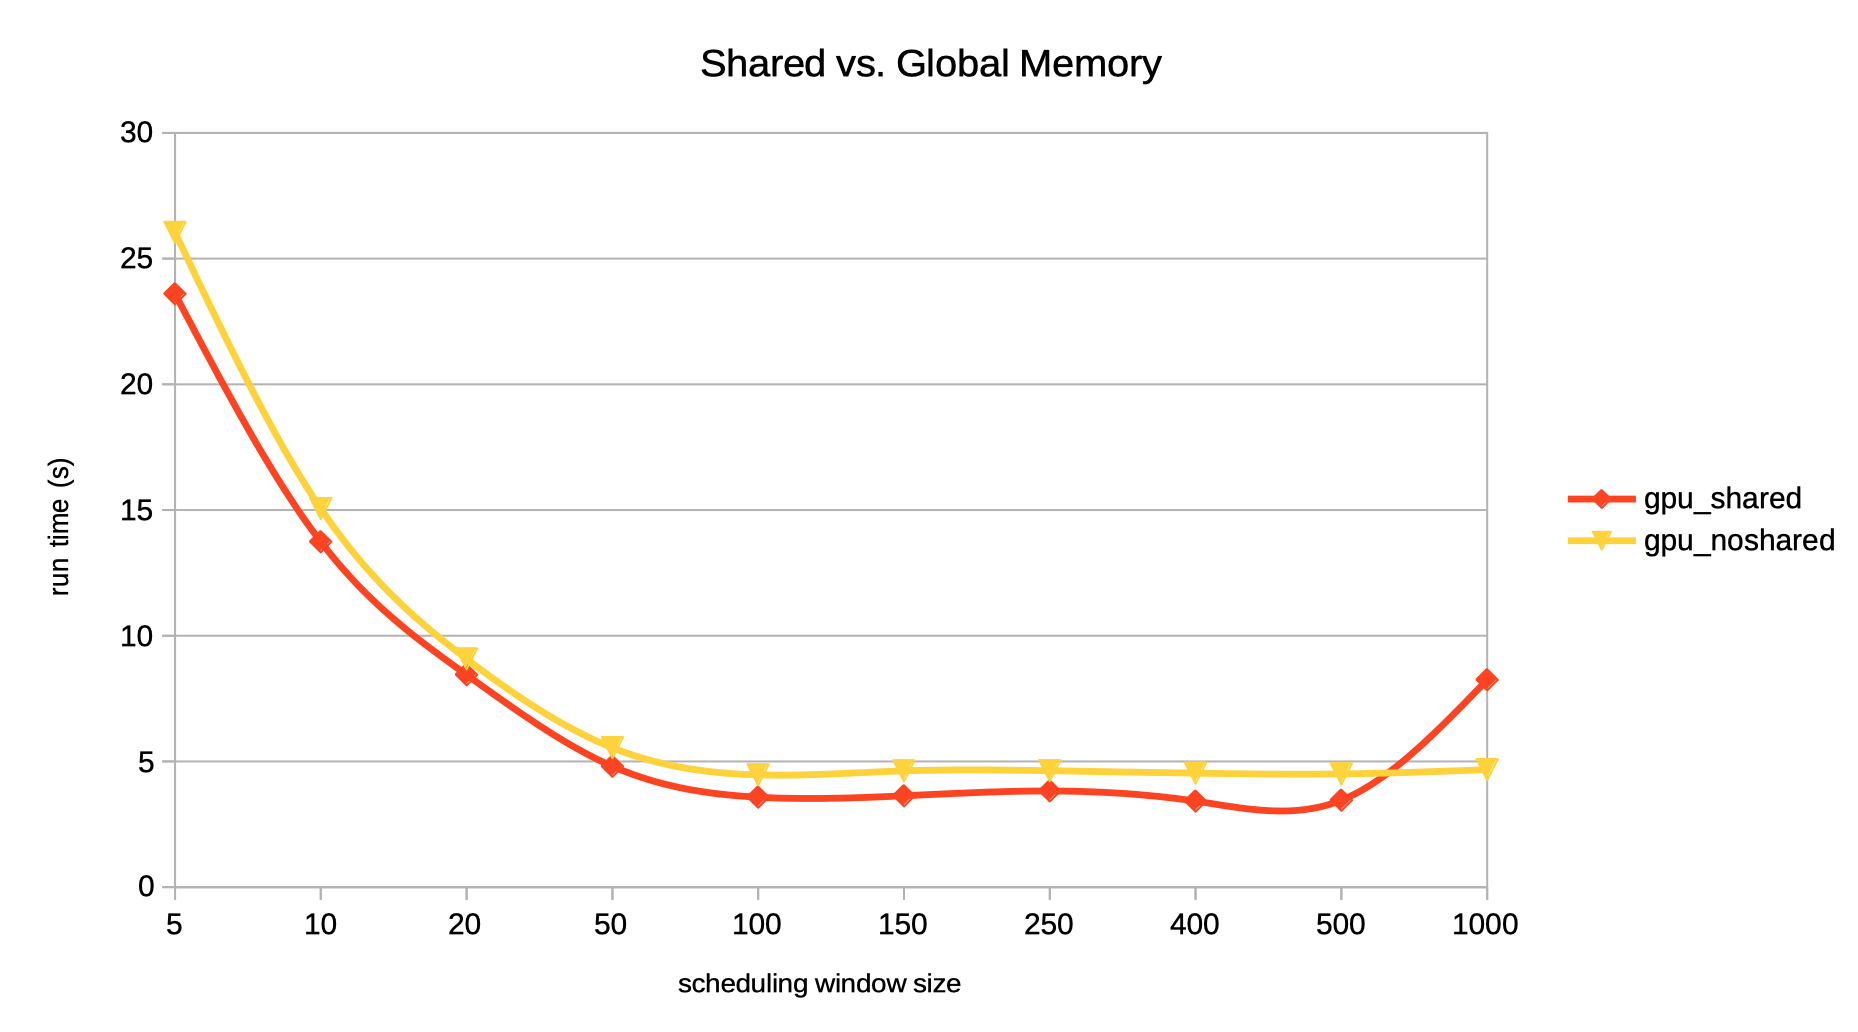
\includegraphics[width=0.5\textwidth]{global_vs_shared}
\caption{Speedup analysis of both implementations: global memory and shared memory.}
\label{fig:globalvshared}
\end{figure}

As can be seen in Figure \ref{fig:globalvshared}, the two implementations perform similarly with the shared memory version consistently faster. This only changes at the end when the scheduling window size causes the two arrays, $a$ and $b$, to significantly exceed the amount of shared memory proportioned to each block (49 KB available - 128 KB needed). This causes the inverted behavior observed at the  scheduling window size of 1000.

Figures \ref{fig:gpu_noshared_time} and \ref{fig:gpu_shared_time} show the time percentages taken up by different portions of code. As can be seen, these are significantly different than Figure \ref{fig:cpu_time}. The CPU no longer takes up 98\% of the algorithm's time. The GPU is able to perform much more work in a lot less time by leveraging millions of concurrent threads.

\begin{figure}[ht]
\centering
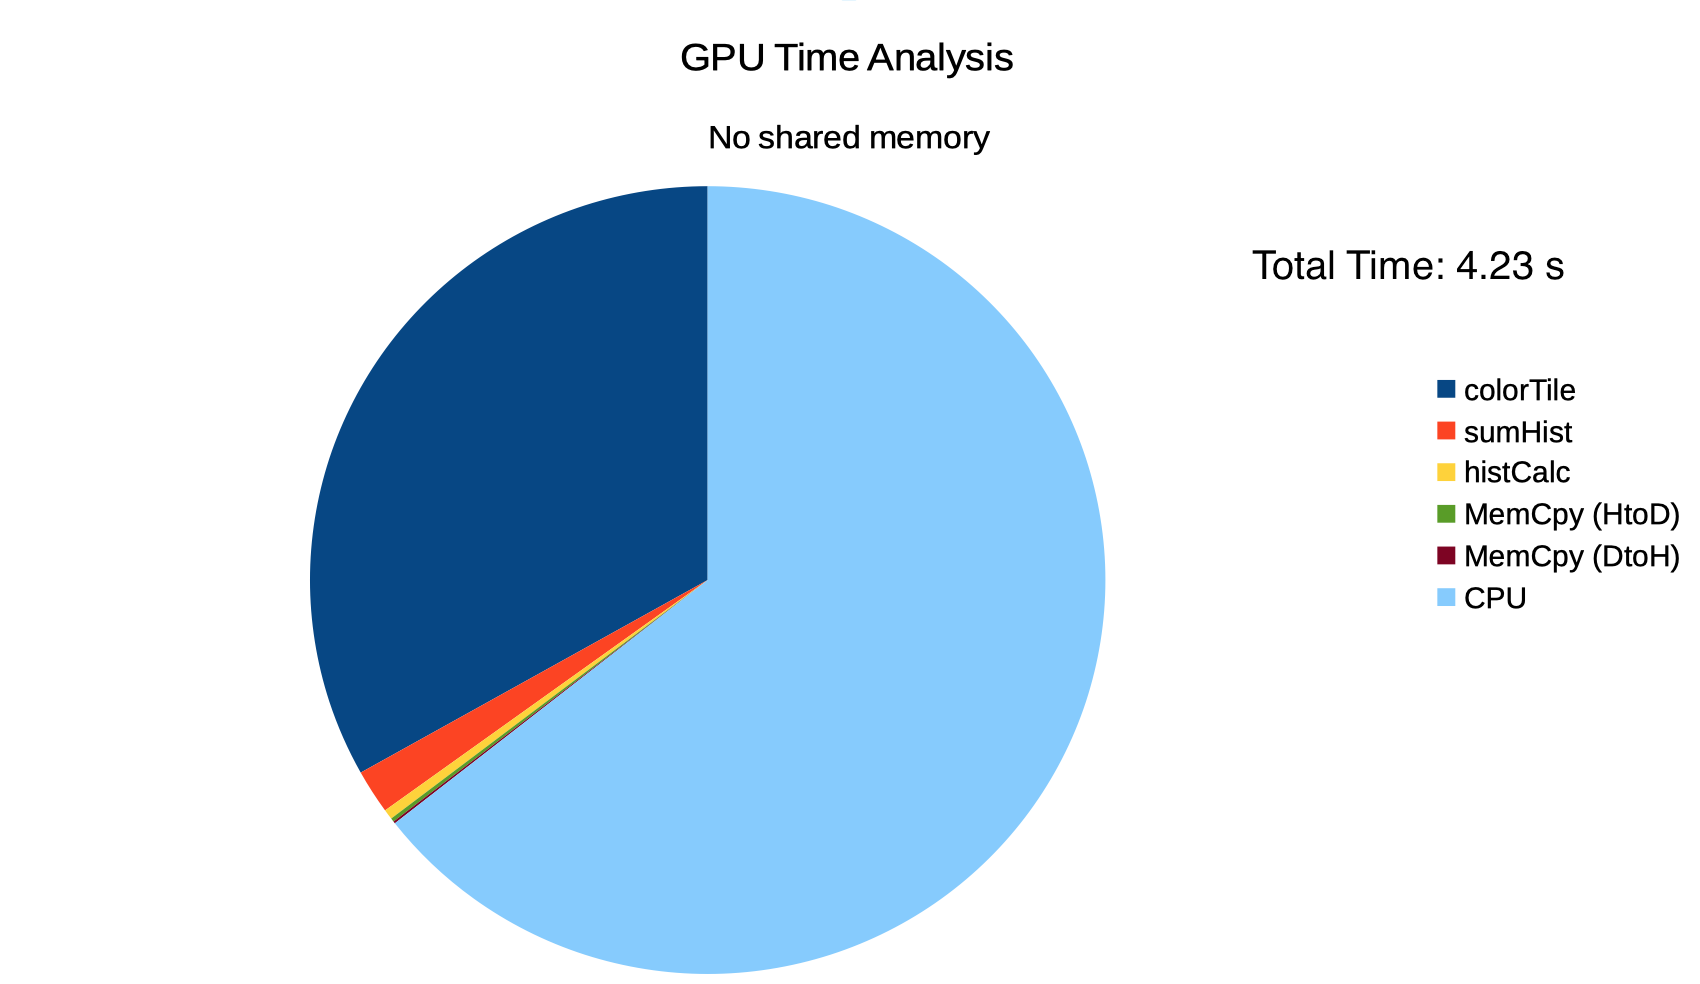
\includegraphics[width=0.5\textwidth]{gpu_noshared_time_analysis}
\caption{Time analysis of GPU implementation without shared memory.}
\label{fig:gpu_noshared_time}
\end{figure}

\begin{figure}[ht]
\centering
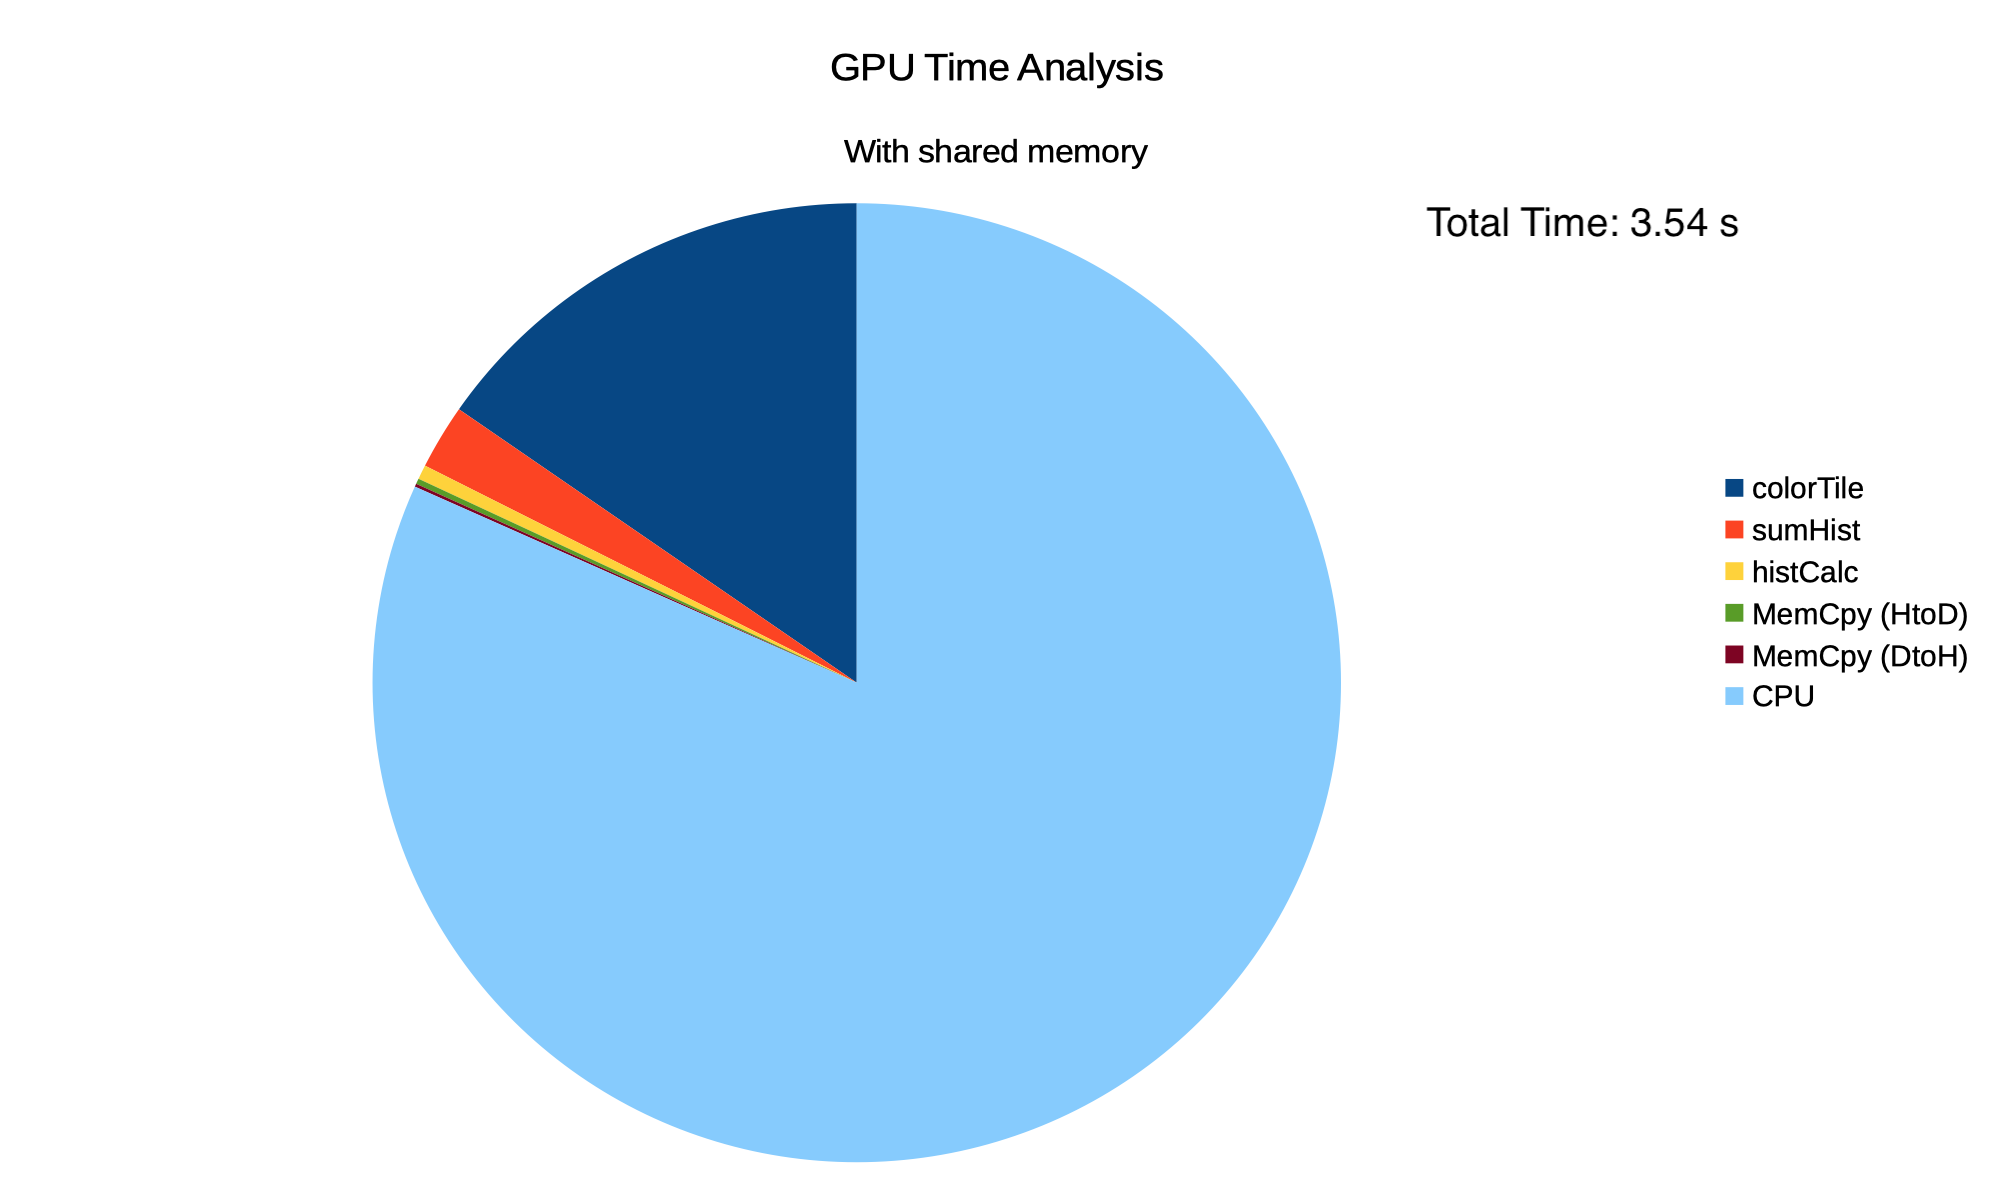
\includegraphics[width=0.5\textwidth]{gpu_shared_time_analysis}
\caption{Time analysis of GPU implementation with shared memory.}
\label{fig:gpu_shared_time}
\end{figure}


\section{Speedup Analysis}

Figure \ref{fig:speedup} shows the CPU and GPU with shared memory implementations side by side with the associated speedup measurement with varying scheduling window size. As shown, the CPU performs well on very small window sizes. This is expected as the amount of parallelization is proportional to the window size. As scheduling window size increases, the GPUs ability to expoit parallelism becomes evident with massive speedup over the CPU implementation. The run time of the CPU version seems to increase exponentially with scheduling window size whereas the GPU version run time remains relatively constant at large window sizes.
%
\begin{figure}[ht]
\centering
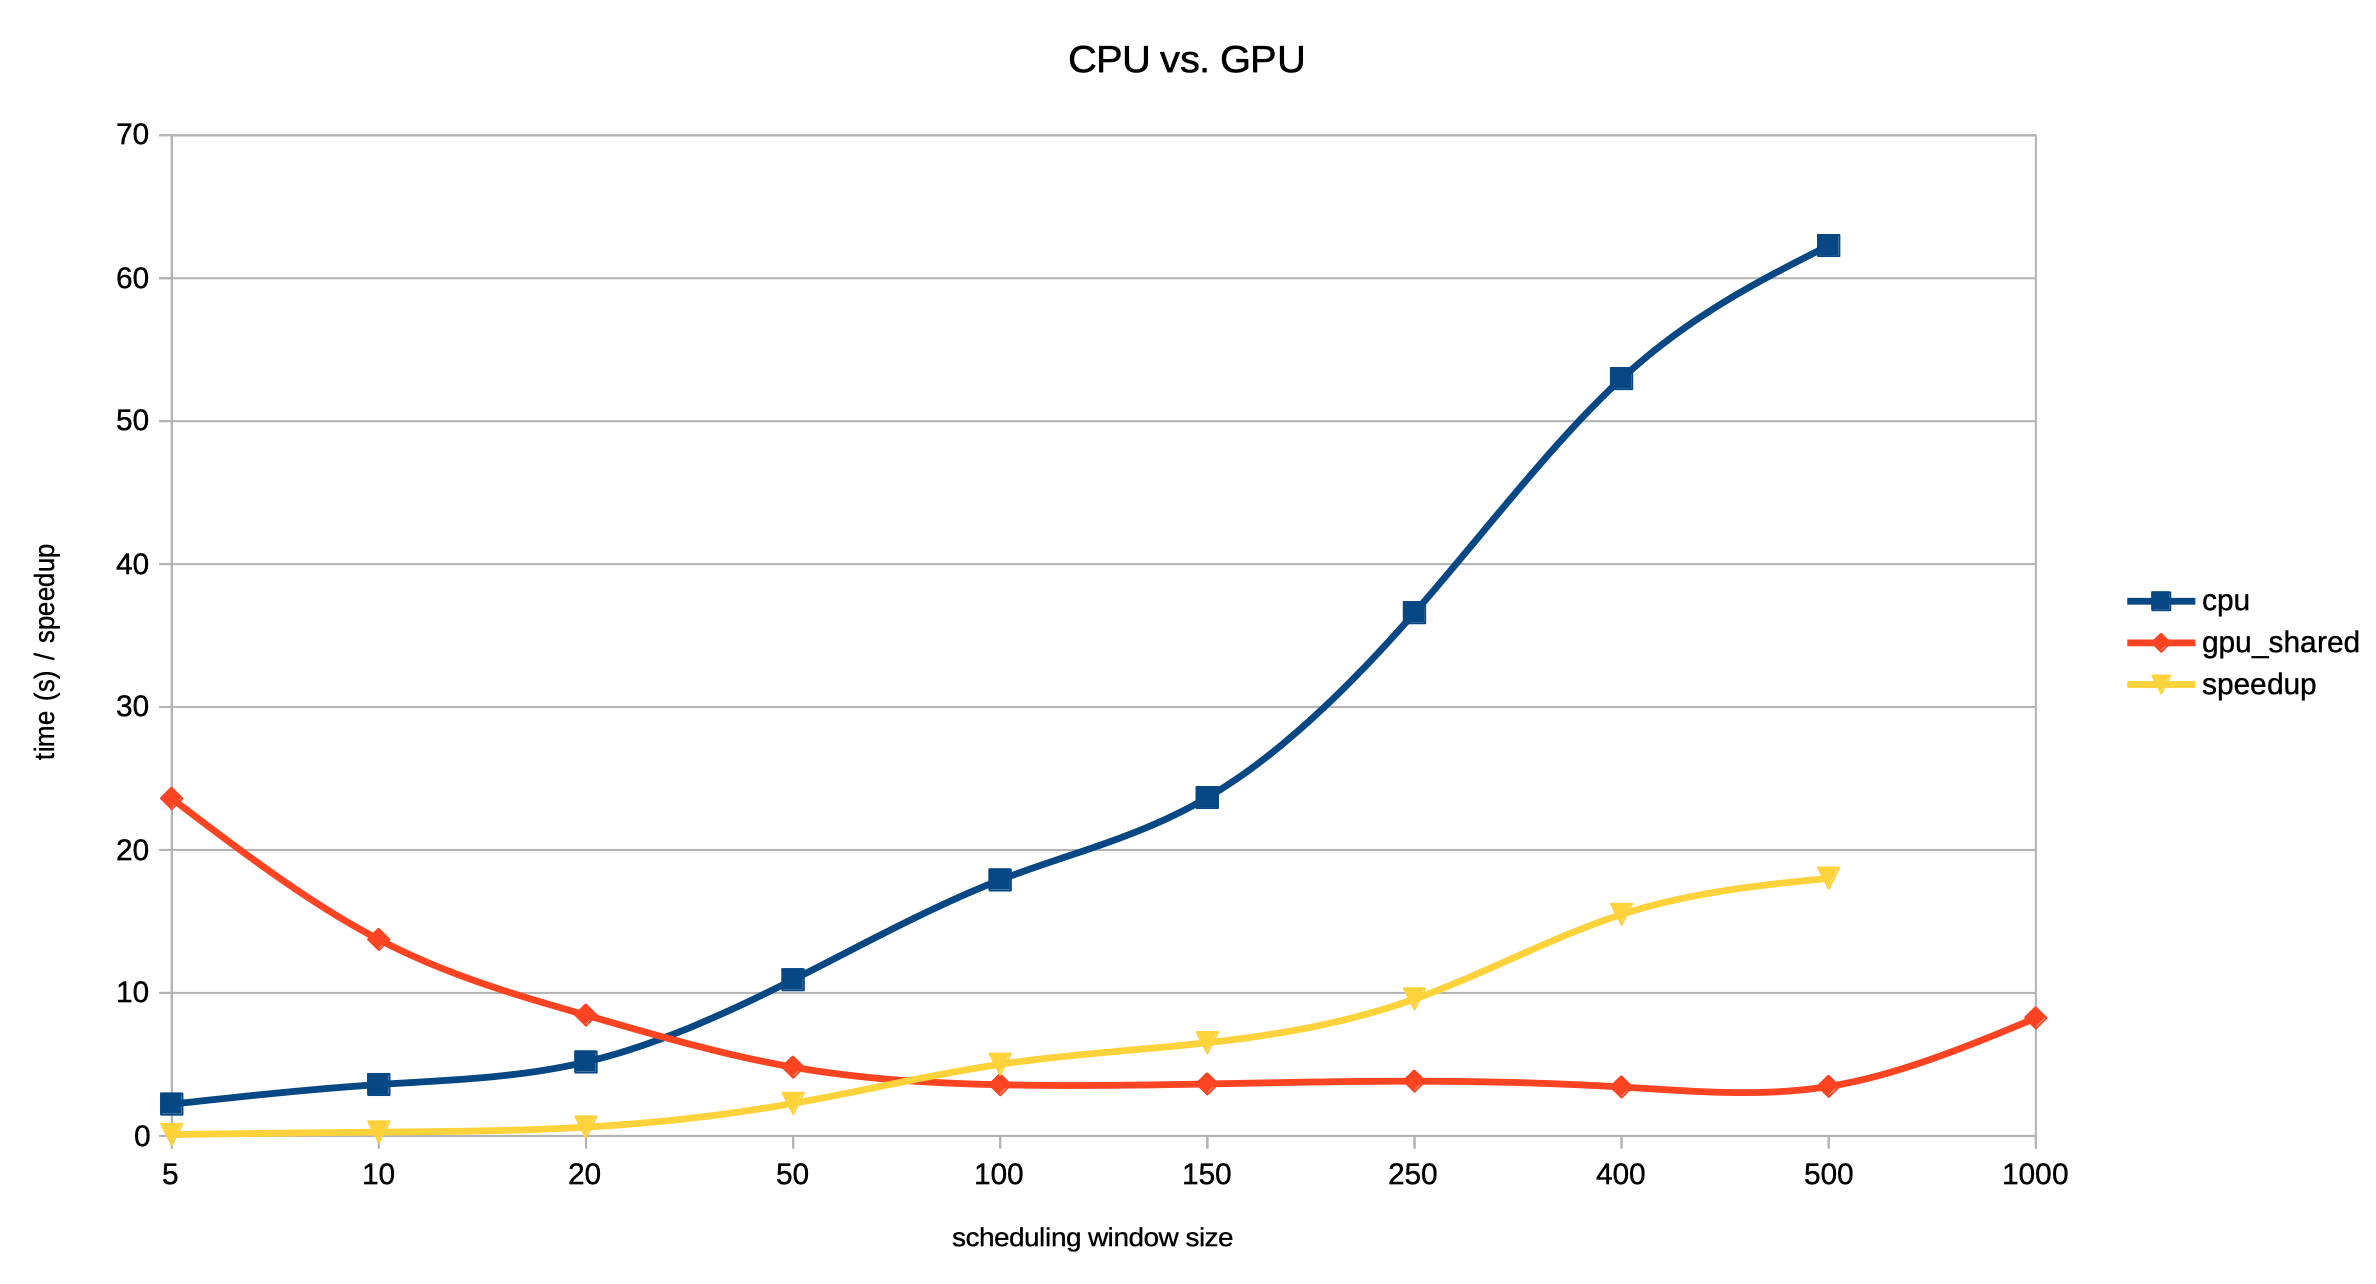
\includegraphics[width=0.5\textwidth]{speedup_graph}
\caption{Speedup analysis of CPU and GPU with shared memory implementations.}
\label{fig:speedup}
\end{figure}
%
\section{Results and Conclusion}

As shown by Table \ref{tab:runtime}, the GPU implementations provide significant speedup by efficiently exploiting the potential parallelism in the tile coloring problem. The use of shared memory further increases the efficiency by reducing the amount of time spent waiting for memory accesses.

\begin{table}[ht]
\renewcommand{\arraystretch}{1.3}
\caption{Run times: scheduling window size of 256.}
\label{tab:runtime}
\centering
\begin{tabular}{|c|c|c|}
  CPU & GPU Global & GPU Shared \\
\hline
  34.48 s & 4.23 s & 3.54 s \\
\end{tabular}
\end{table}


\newpage
\appendices
\section{Device Query Results}
\VerbatimInput{../part1/deviceQueryResults.txt}
\section{Bandwidth Test}
\VerbatimInput{../part1/bandwidthTest.txt}


\newpage

% \bibliographystyle{IEEEtran}
% \bibliography{ref}

\end{document}
